\documentclass[12pt,a4paper,headings=optiontohead]{article}
\usepackage[utf8]{inputenc}
\usepackage[italian]{babel}
\usepackage[margin=1.8cm,bottom=7em]{geometry}
\usepackage[subpreambles=false]{standalone}
\usepackage{amsmath}
\usepackage{amssymb}
\usepackage{amsthm} 
\usepackage{cancel}
\usepackage{hyperref}
\usepackage{graphicx}
\usepackage{mathtools}
\usepackage{float}
\usepackage{enumitem}
\usepackage{pdfpages}
\usepackage[normalem]{ulem}

\usepackage{blkarray}% http://ctan.org/pkg/blkarray

\newcommand{\matindex}[1]{\mbox{\scriptsize#1}}% Matrix index

\renewcommand{\qedsymbol}{\rule{0.7em}{0.7em}}
\DeclarePairedDelimiter{\abs}{\lvert}{\rvert}
\newcommand{\inter}{\begin{matrix}\prod\end{matrix}}
\newcommand{\verteq}{\rotatebox{90}{$\,=$}}
\newcommand{\equalto}[2]{\underset{\scriptstyle\overset{\mkern4mu\verteq}{#2}}{#1}}
\DeclarePairedDelimiter{\norma}{\lVert}{\rVert}
\newtheorem*{esempio}{Esempio}

\usepackage{import}
\usepackage{hyperref}
\begin{document}

%------------------------------------------------------------------------------------------------------
%------------------------------------------------------------------------------------------------------
%-----------------------------------------------INTESTAZIONE-------------------------------------------
%------------------------------------------------------------------------------------------------------
%------------------------------------------------------------------------------------------------------

\begin{titlepage}

\newcommand{\HRule}{\rule{\linewidth}{0.5mm}} % Defines a new command for the horizontal lines, change thickness here

\center % Center everything on the page
 
%----------------------------------------------------------------------------------------
%	HEADING SECTIONS
%----------------------------------------------------------------------------------------


%----------------------------------------------------------------------------------------
%	TITLE SECTION
%----------------------------------------------------------------------------------------

\HRule \\[0.4cm]
{ \huge \bfseries UltimateCN}\\
\HRule \\[1.5cm]
 
%----------------------------------------------------------------------------------------
%	AUTHOR SECTION
%----------------------------------------------------------------------------------------


%----------------------------------------------------------------------------------------
%	DATE SECTION
%----------------------------------------------------------------------------------------

\LARGE Università degli Studi di Padova\\[0.4cm] % Name of your university/college
{\large Dipartimento di Matematica}\\[0.05cm]
\textsc{\large Corso di Laurea in Informatica}\\[1cm] % Include a department/university logo - this will require the graphicx package

{\Large Anno accademico 2022 - 2023}\\[2cm] % Date, change the \today to a set date if you want to be precise
\begin{minipage}{0.4\textwidth}
	\begin{flushleft} \large
		\emph{\Large{Autore:}}\\
		\quad \quad \textsc{Nicola Baesso}
	\end{flushleft}
	
\end{minipage}\\[3cm]

\vfill % Fill the rest of the page with whitespace

\end{titlepage}


\begin{center}
\pagebreak

\section*{Premessa}
\begin{minipage}{0.9\textwidth} \large

Questa raccolta é stata ispirata dal giá ottimo documento "Calcolo Numerico Completo", e vuole estendere in maniera completa quanto presente.\\\\
La repository in cui segnalare problematiche o suggerire modifiche tramite PR si puo' trovare qui: \href{https://github.com/nicolabaesso/UltimateCN}{https://github.com/nicolabaesso/UltimateCN}

\end{minipage}

\end{center}
\pagebreak

%------------------------------------------------------------------------------------------------------
%------------------------------------------------------------------------------------------------------
%-----------------------------------------------INDICE-------------------------------------------------
%------------------------------------------------------------------------------------------------------
%------------------------------------------------------------------------------------------------------

\tableofcontents
\section{Quiz parte teorica}
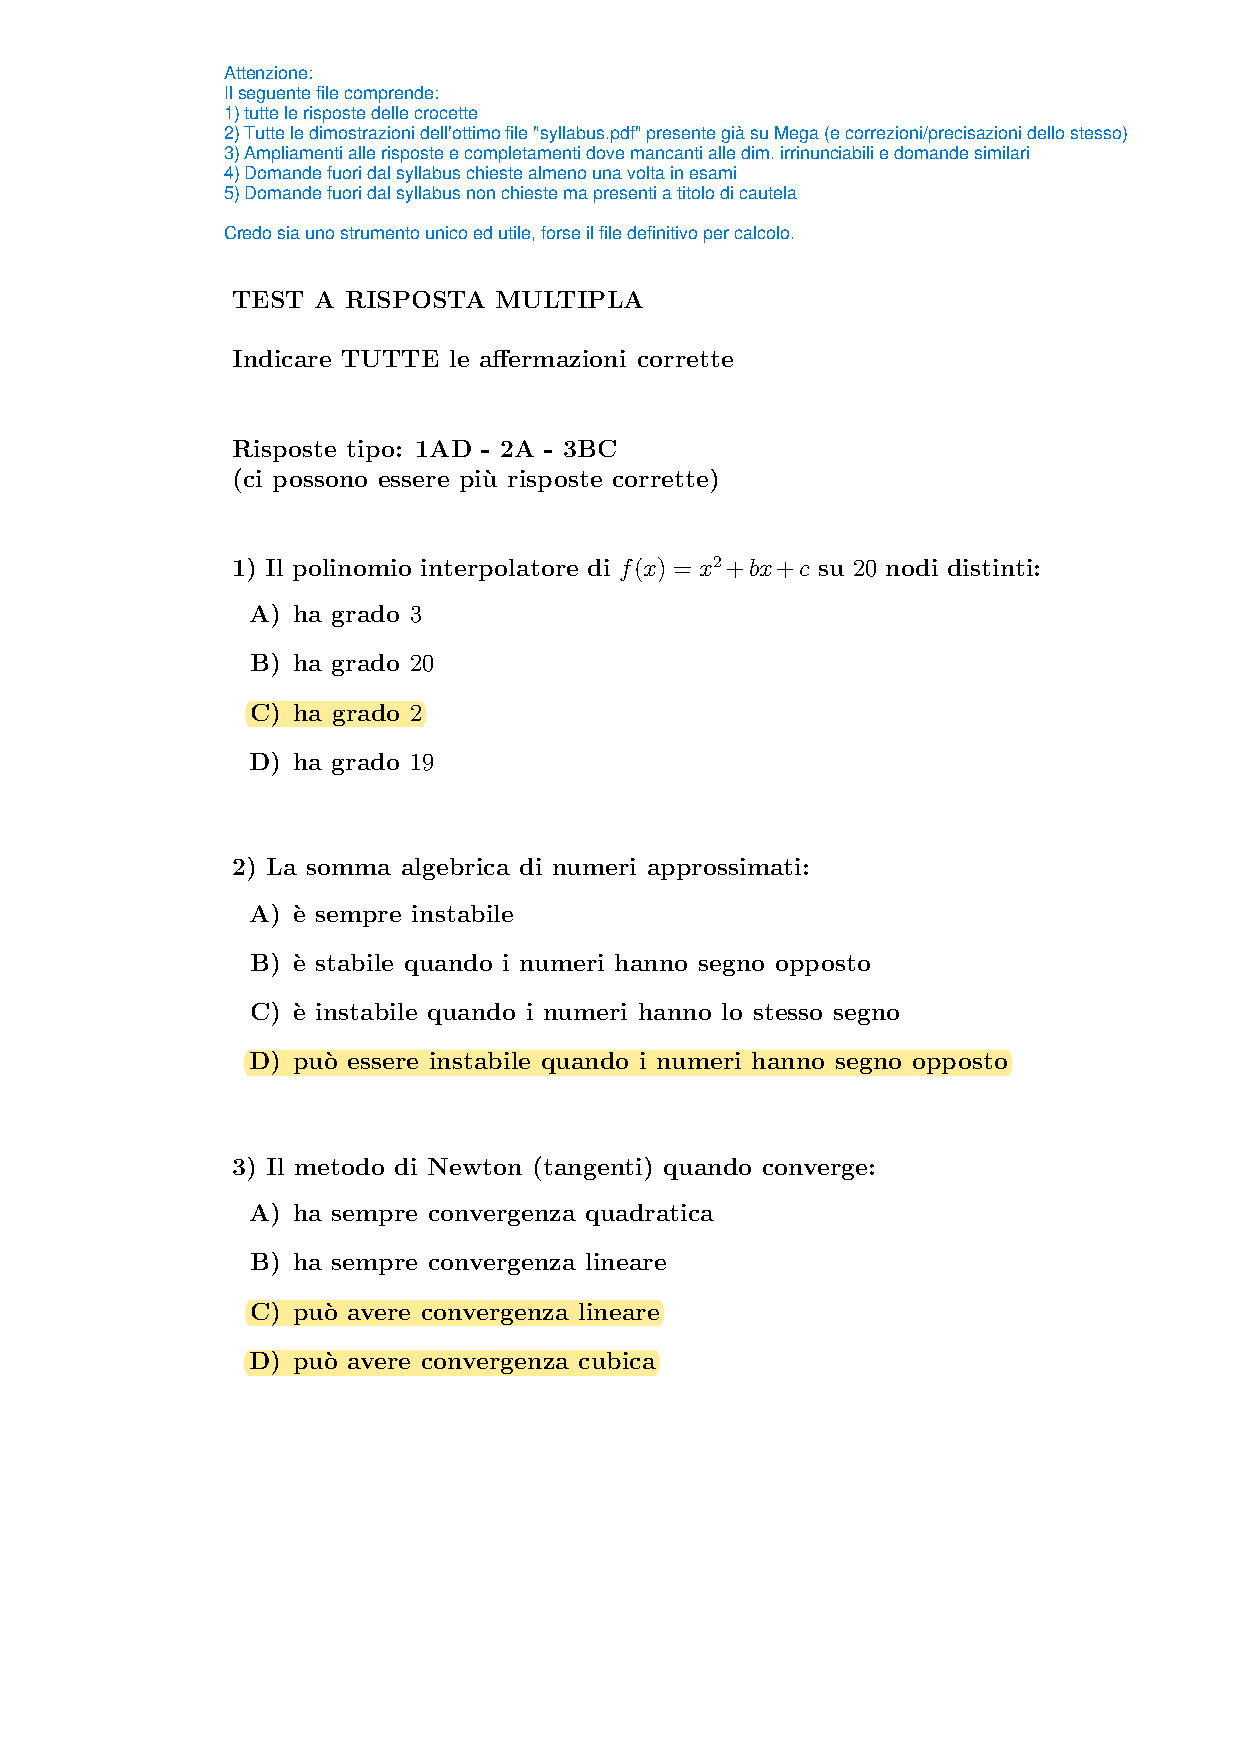
\includepdf[pages={1-8}]{Calcolo_Completo.pdf}
\section{Dimostrazioni irrinunciabili}
\import{res/}{precis_macchina}
\newpage
\import{res/}{analisi_stab}
\import{res/}{conv_bisez}
\newpage
\import{res/}{stima_err_res_pesato}
\newpage
\import{res/}{conv_newton}
\newpage
\import{res/}{vel_conv}
\newpage
\import{res/}{ord_conv_pt_fisso}
\newpage
\import{res/}{esis_unix_inter_polin}
\newpage
\import{res/}{inter_lin_tratti}
\newpage
\import{res/}{stima_eq_normali}
\newpage
\import{res/}{stima_cond_sist_lineare}
\newpage
\section{Dimostrazioni facoltative}
\end{document}
